\documentclass{standalone}
\usepackage{tikz}
% put any importmodules into the preamble
\begin{document}
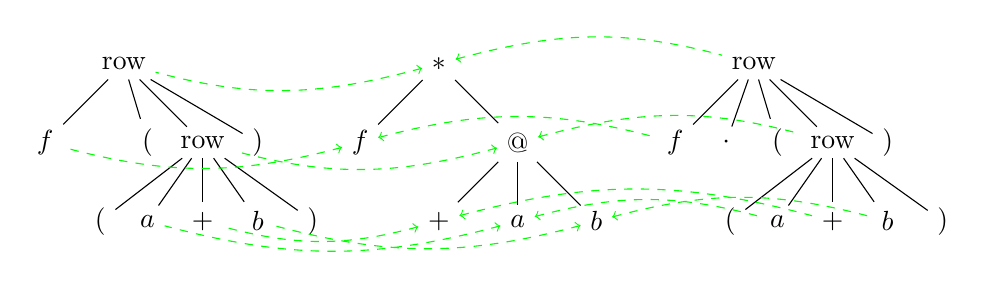
\begin{tikzpicture} 
% product 
\node (c1f) at (4,1) {$f$};
\node (c1a1) at (5,2) {$*$};
\node (c1a2) at (6,1) {$@$};
\node (c1p) at (5,0) {$+$};
\node (c1a) at (6,0) {$a$};
\node (c1b) at (7,0) {$b$};
\draw (c1a1) -- (c1f);
\draw (c1a1) -- (c1a2);
\draw (c1a2) -- (c1p);
\draw (c1a2) -- (c1a);
\draw (c1a2) -- (c1b);
% presentation tree
\node (p1f) at (0,1) {$f$};
\node (p1a1) at (1,2) {row};
\node (p1a2o) at (1.3,1) {$($};
\node (p1a2) at (2,1) {row};
\node (p1a2c) at (2.7,1) {$)$};
\node (p1o) at (.7,0) {$($};
\node (p1a) at (1.3,0) {$a$};
\node (p1p) at (2,0) {$+$};
\node (p1b) at (2.7,0) {$b$};
\node (p1c) at (3.4,0) {$)$};
\draw (p1a1) -- (p1f);
\draw (p1a1) -- (p1a2o);
\draw (p1a1) -- (p1a2);
\draw (p1a1) -- (p1a2c);
\draw (p1a2) -- (p1p);
\draw (p1a2) -- (p1a);
\draw (p1a2) -- (p1b);
\draw (p1a2) -- (p1o);
\draw (p1a2) -- (p1c);
\draw[<-,green,dashed] (c1f) to[out=195,in=-15] (p1f);
\draw[<-,green,dashed] (c1a1) to[out=195,in=-15] (p1a1);
\draw[<-,green,dashed] (c1a2) to[out=195,in=-15] (p1a2);
\draw[<-,green,dashed] (c1p) to[out=195,in=-15] (p1p);
\draw[<-,green,dashed] (c1a) to[out=195,in=-15] (p1a);
\draw[<-,green,dashed] (c1b) to[out=195,in=-15] (p1b);
% presentation tree2
\node (p2f) at (8,1) {$f$};
\node (p2t) at (8.65,1) {$\cdot$};
\node (p2a1) at (9,2) {row};
\node (p2a2o) at (9.3,1) {$($};
\node (p2a2) at (10,1) {row};
\node (p2a2c) at (10.7,1) {$)$};
\node (p2o) at (8.7,0) {$($};
\node (p2a) at (9.3,0) {$a$};
\node (p2p) at (10,0) {$+$};
\node (p2b) at (10.7,0) {$b$};
\node (p2c) at (11.4,0) {$)$};
\draw (p2a1) -- (p2f);
\draw (p2a1) -- (p2t);
\draw (p2a1) -- (p2a2o);
\draw (p2a1) -- (p2a2);
\draw (p2a1) -- (p2a2c);
\draw (p2a2) -- (p2p);
\draw (p2a2) -- (p2a);
\draw (p2a2) -- (p2b);
\draw (p2a2) -- (p2o);
\draw (p2a2) -- (p2c);
\draw[<-,green,dashed] (c1f) to[out=15,in=165] (p2f);
\draw[<-,green,dashed] (c1a1) to[out=15,in=165] (p2a1);
\draw[<-,green,dashed] (c1a2) to[out=15,in=165] (p2a2);
\draw[<-,green,dashed] (c1p) to[out=15,in=165] (p2p);
\draw[<-,green,dashed] (c1a) to[out=15,in=165] (p2a);
\draw[<-,green,dashed] (c1b) to[out=15,in=165] (p2b);
\end{tikzpicture}
\end{document}
%%% Local Variables: 
%%% mode: latex
%%% TeX-master: t
%%% End: 
